\documentclass{article}
\usepackage[utf8]{inputenc}
\usepackage{polski}
\usepackage{geometry}
\usepackage{pdfpages}
\usepackage{pdfpages}
\usepackage{listings}
\usepackage{listingsutf8}
\usepackage{multirow}
\usepackage{siunitx}
\usepackage{multirow}
\usepackage{booktabs}
\usepackage{tabularx}
\usepackage{placeins}
\usepackage{pdflscape}
\usepackage{graphicx}
\usepackage{subfig}
\usepackage{hyperref}
\usepackage{amsmath}
\usepackage{colortbl}

\geometry{
a4paper,
total={170mm,257mm},
left=20mm,
top=20mm
}
\newcolumntype{Y}{>{\centering\arraybackslash}X}
\renewcommand\thesection{}
\lstset{%
literate=%
 {ą}{{\k{a}}}1
 {ę}{{\k{e}}}1
 {Ą}{{\k{A}}}1
 {Ę}{{\k{E}}}1
 {ś}{{\'{s}}}1
 {Ś}{{\'{S}}}1
 {ź}{{\'{z}}}1
 {Ź}{{\'{Z}}}1
 {ń}{{\'{n}}}1
 {Ń}{{\'{N}}}1
 {ć}{{\'{c}}}1
 {Ć}{{\'{C}}}1
 {ó}{{\'{o}}}1
 {Ó}{{\'{O}}}1
 {ż}{{\.{z}}}1
 {Ż}{{\.{Z}}}1
 {ł}{{\l{}}}1
 {Ł}{{\l{}}}1
}

\title{Metody Obliczeniowe w Nauce i Technice\\ 
Laboratorium IV}
\author{Maciej Trątnowiecki}
\date{AGH, Semestr Letni, 2020}

\begin{document}
    \maketitle
    \section{Problem komiwojażera}
        W ramach zadania zaimplementowałem program szukający optymalnej ścieżki w problemie komiwojażera dla losowych punktów na płaszczyźnie dwuwymiarowej. Przetestowałem go dla punktów losowanych z rozkładu jednostajnego, normalnego i podzielonych na 9 odseparowanych grup. 
        
        
        Przykładowe wyniki działania programu:
        % n100 t20 uni : 25.52 %
        % n500 t20 uni: 20.72%
        % n 1000 t31 uni : 20.69%

        \begin{figure}[h!]
            \centering
            \subfloat[]{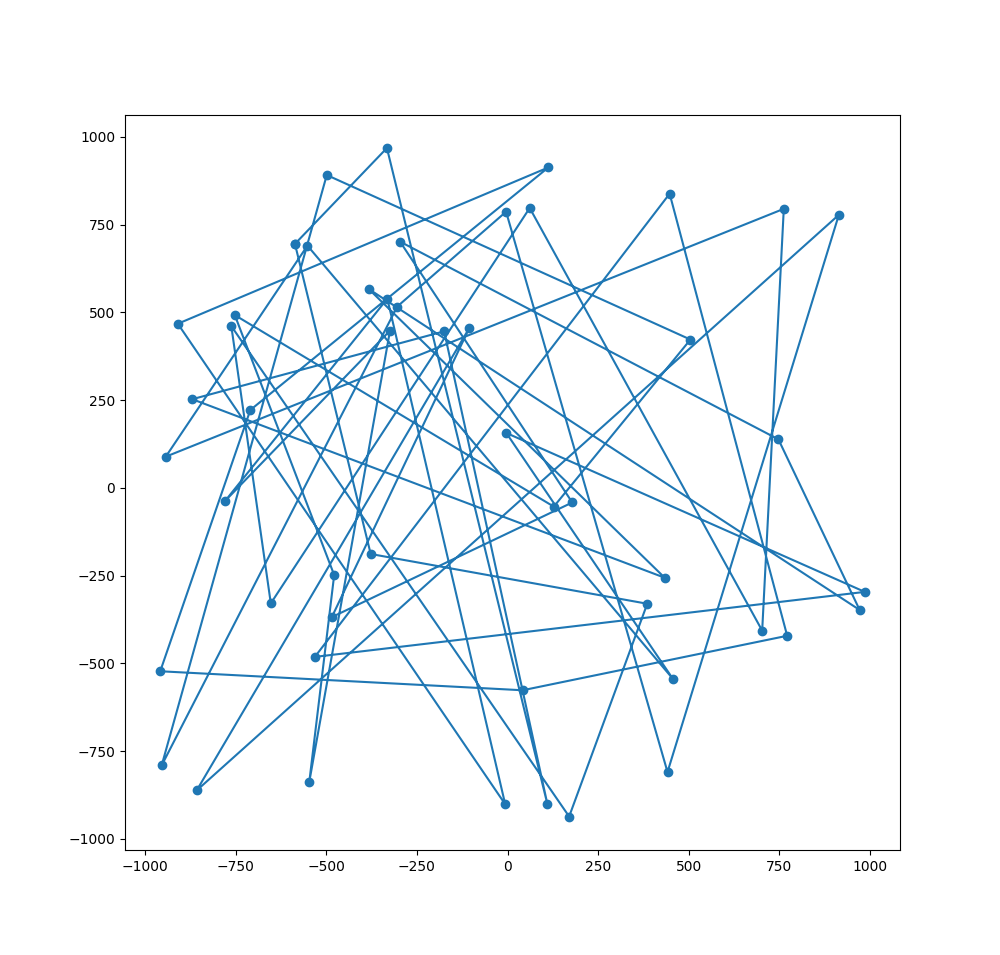
\includegraphics[width=6cm]{lab4/img/tsp_n100_t20_uni_pre.png}}
            \subfloat[]{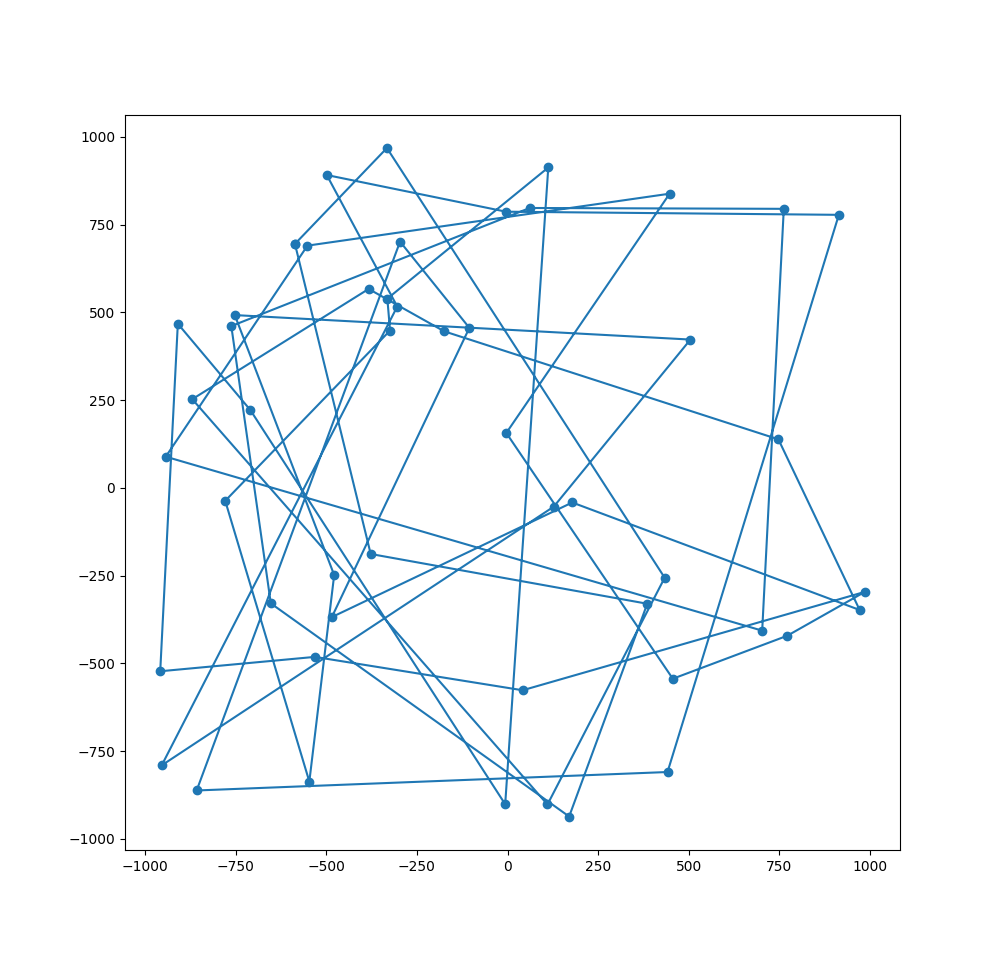
\includegraphics[width=6cm]{lab4/img/tsp_n100_t20_uni_post.png}}
            \subfloat[]{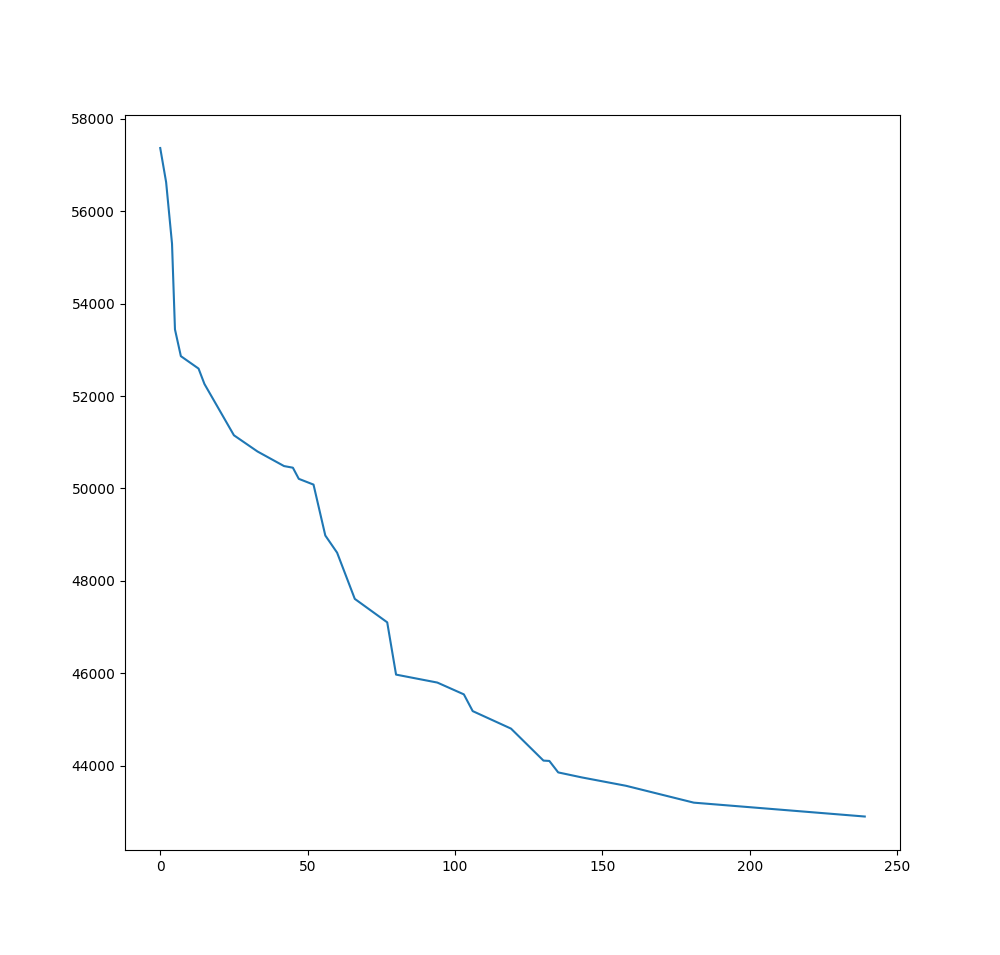
\includegraphics[width=6cm]{lab4/img/tsp_n100_t20_uni_plot.png}}
            \caption{Rozkład jednostajny, $100$ punktów, temperatura $20$, optymalizacja trasy $25.52\%$}
        \end{figure}\\
        \begin{figure}[h!]
            \centering
            \subfloat[]{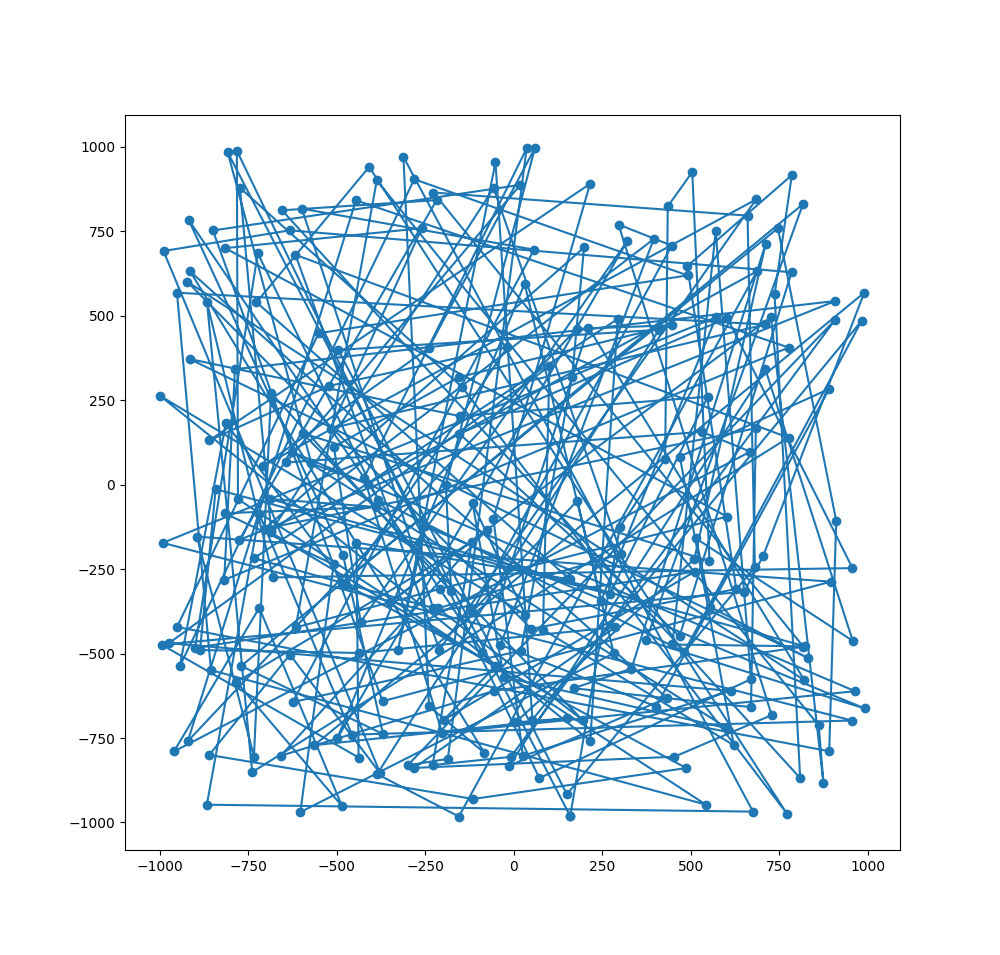
\includegraphics[width=6cm]{lab4/img/tsp_n500_t20_uni_pre.png}}
            \subfloat[]{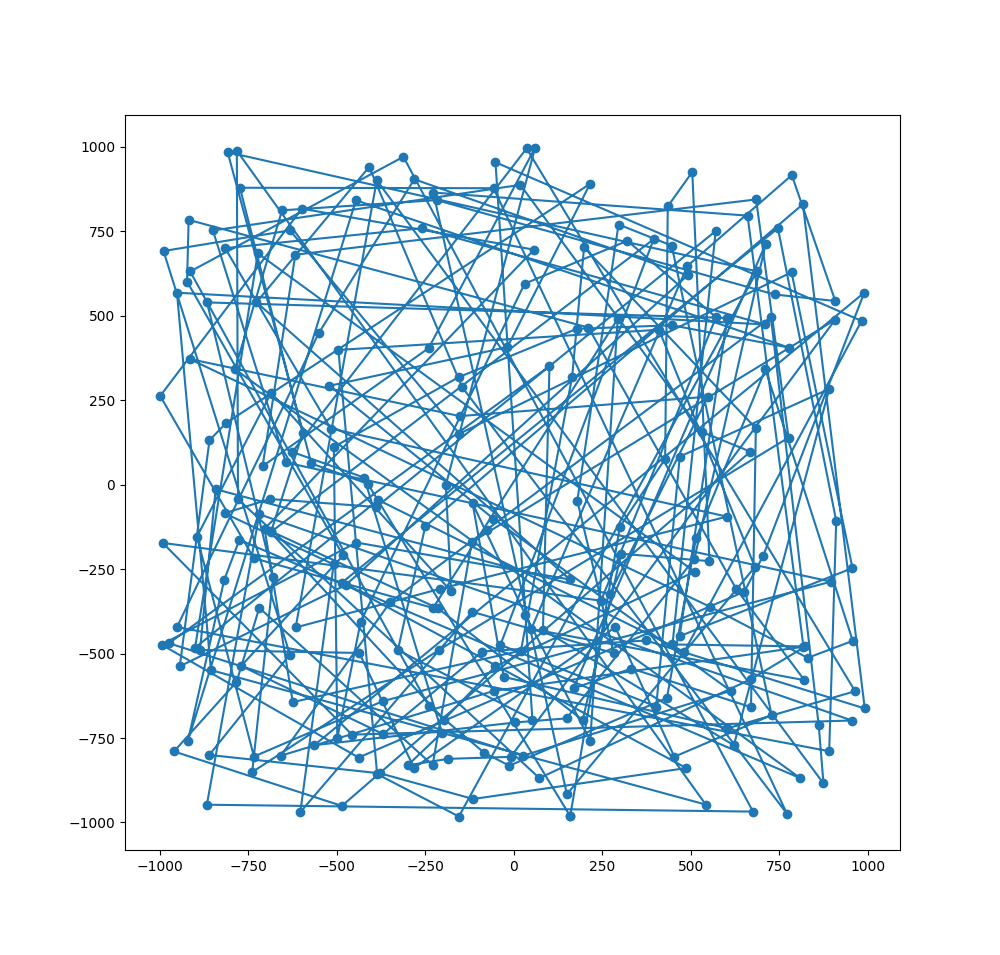
\includegraphics[width=6cm]{lab4/img/tsp_n500_t20_uni_post.png}}
            \subfloat[]{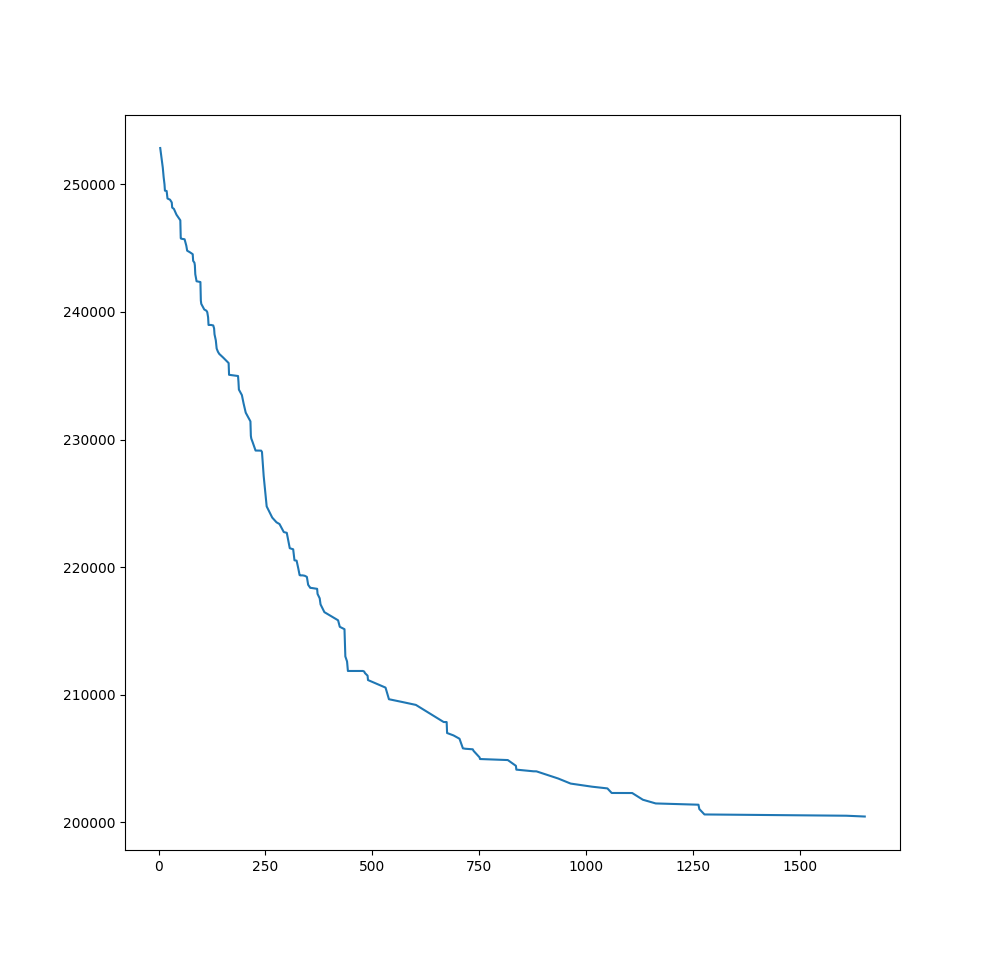
\includegraphics[width=6cm]{lab4/img/tsp_n500_t20_uni_plot.png}}
            \caption{Rozkład jednostajny, $500$ punktów, temperatura $20$, optymalizacja trasy $20.72\%$}
        \end{figure}\\
        \begin{figure}[h!]
            \centering
            \subfloat[]{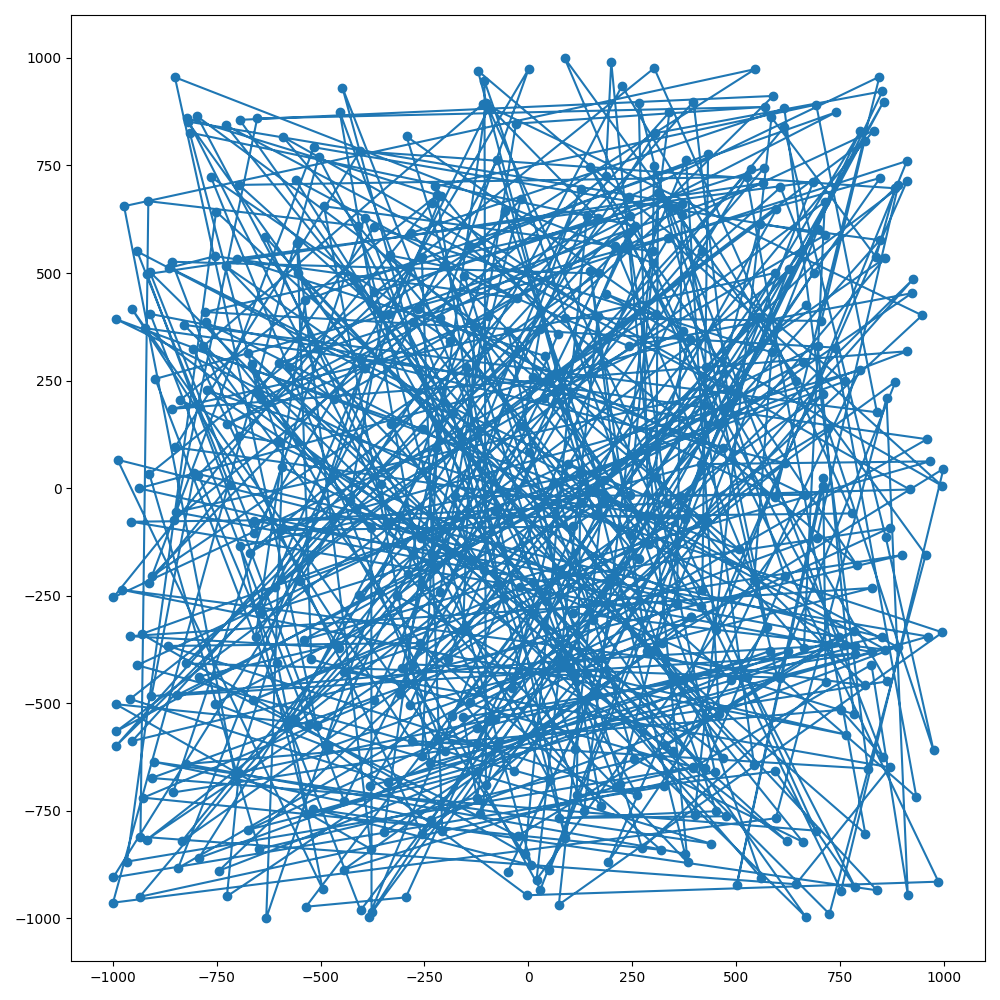
\includegraphics[width=6cm]{lab4/img/tsp_n1000_t31_uni_pre.png}}
            \subfloat[]{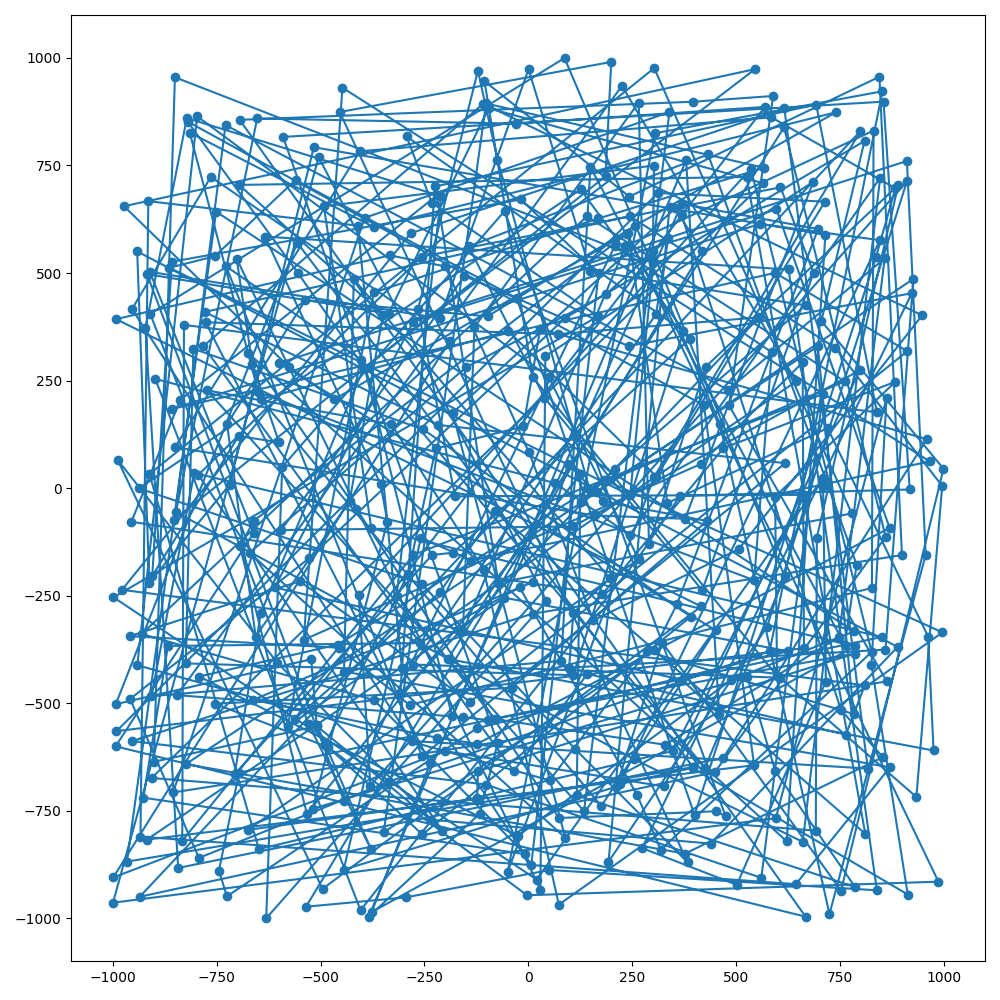
\includegraphics[width=6cm]{lab4/img/tsp_n1000_t31_uni_post.png}}
            \subfloat[]{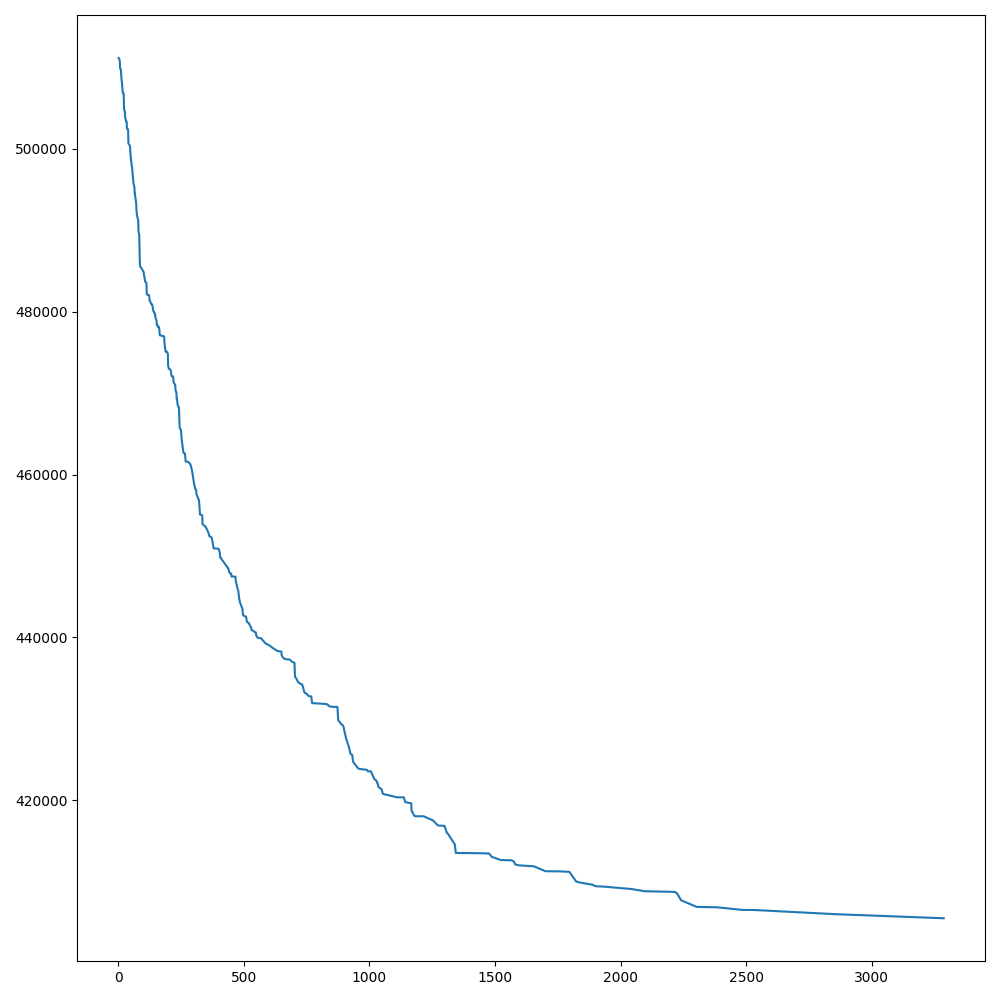
\includegraphics[width=6cm]{lab4/img/tsp_n1000_t31_uni_plot.png}}
            \caption{Rozkład jednostajny, $1000$ punktów, temperatura $31$, optymalizacja trasy $20.69\%$}
        \end{figure}\\
        

\end{document}